\documentclass{article}
\usepackage[a4paper, total={6in, 10in}]{geometry}
\usepackage{mymath}

\title{Variational Inference and Variational Auto-Encoder}
\author{Jingfeng Wu}
\date{Created: March 2018\\ Last updated: \today}

\begin{document}
\maketitle
For more details, please refer to~\cite{blei2017variational,doersch2016tutorial,kingma2013autoencoding,kingma2019introduction}.

\section{Variational Inference}
Let $X = \{x_i\}_{i=1}^N$ be a set of observed data.
In Variational Inference (VI), we want to approximate a complicated and intractable conditional distribution $P(z|X)$ with some simple and tractable distribution $Q(z; \upsilon)$ parameterized by $\upsilon$.
Here we do not write the dependence of $Q(z;\upsilon)$ on $X$ explicitly, since $X$, the observed data, is fixed.
$Q(z;\upsilon)$ can be replaced with a conditional distribution when one assumes $X$ is variable and drawn from some distribution.

First one can easily obtain that
\begin{equation}
    \kld{Q(z;\upsilon)}{P(z|X)} = \sum_{z}Q(z;\upsilon) \log \frac{Q(z;\upsilon)}{P(z|X)} = \log P(X) + \sum_{z} Q(z;\upsilon) \log \frac{Q(z;\upsilon)}{P(z,X)}.
\end{equation}
Note that $\log P(X)$ is fixed since $X$ is given.
Suppose the desired conditional distribution $P(z|X)$ is not that complicated, and our model $Q(z;\upsilon)$ is flexible enough such that $Q(z;\upsilon^*) = P(z|X)$ for $\upsilon^* = \argmin_{\upsilon} \kld{Q(z;\upsilon)}{P(z|X)}$.
Thus by taking minimization with respect to $\upsilon$ in both sides, we have
\begin{equation}
    0 = \min_{\upsilon}\kld{Q(z;\upsilon)}{P(z|X)} = \log P(X) + \min_{\upsilon}\sum_{z} Q(z;\upsilon) \log \frac{Q(z;\upsilon)}{P(z,X)}.
\end{equation}
Thus
\begin{equation}\label{eq:vi}
    \log P(X) = \max_{\upsilon} - \sum_{z} Q(z;\upsilon) \log \frac{Q(z;\upsilon)}{P(z,X)}.
\end{equation}
The key ingredient in VI is to smartly model the distributions such that the right hand side of Eq.~\eqref{eq:vi} is tractable.


\section{Variational Auto-Encoder}
For an example of VI, let us elaborate Variational Auto-Encoder (VAE)~\cite{kingma2013autoencoding}.
Suppose we have observed a dataset $X = \{x_i\}_{i=1}^N$, and we aim to learn its distribution, i.e. we want to maximize the log-likelihood over the observed data,
\begin{equation}\label{eq:mle}
    \max_{\theta}\Ebb_{x\in X}\log P(x;\theta).
\end{equation}
Now let us introduce $Q(z|x;\upsilon)$ to approximate $P(z|x;\theta)$.
By VI~\eqref{eq:vi}, we have
\begin{equation}
\begin{aligned}
    \log P(x;\theta) 
    =& \max_{\upsilon} - \sum_{z} Q(z|x;\upsilon) \log \frac{Q(z|x;\upsilon)}{P(z,x;\theta)} \\
    =& \max_{\upsilon} \sum_{z}Q(z|x,\upsilon)\log P(x|z;\theta) - \kld{Q(z|x;\upsilon)}{P(z; \theta)}
\end{aligned}
\end{equation}
Thus the maximum log-likelihood~\eqref{eq:mle} becomes
\begin{equation}\label{eq:vae-loss}
    \max_{\theta}\Ebb_{x\in X}\log P(x;\theta) = \max_{\theta, \upsilon} \Ebb_{x\in X}\sum_{z}Q(z|x,\upsilon)\log P(x|z;\theta) - \kld{Q(z|x;\upsilon)}{P(z; \theta)}
\end{equation}

Let $A = \sum_{z}Q(z|x,\upsilon)\log P(x|z;\theta)$ and $B = \kld{Q(z|x;\upsilon)}{P(z; \theta)}$.
In order to optimization the VAE loss~\eqref{eq:vae-loss}, it remains to show how to compute the right hand side of Eq.~\eqref{eq:vae-loss}, i.e., $A$ and $B$.

\subsection{The reparameterization trick}
Notice that $A = \Ebb_{z\sim Q(z|x,\upsilon)}\log P(x|z;\theta)$ is an expectation over some hidden random variable $z$.
The optimization of $\theta$ can be done with Monte-Carlo estimation and typical gradient descent (or its variants).
Generally, however, it is intractable to calculate the gradient on $\upsilon$ since a random variable $z$ is not differentiable.
The solution to this challenge involves an important trick called \emph{the reparameterization trick}.
See Figure~\ref{fig:vae} for some intuition.

\begin{figure}
\centering
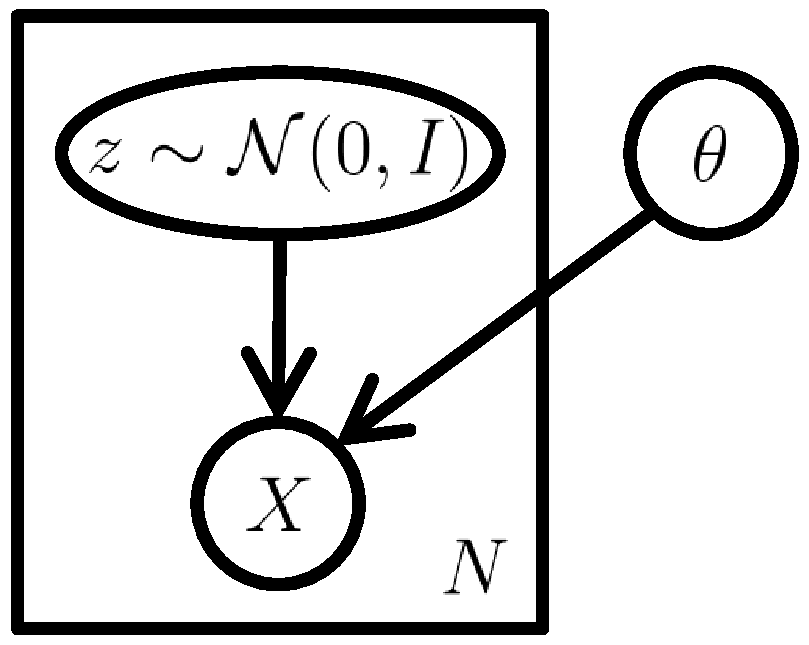
\includegraphics[width=0.3\textwidth]{figures/graphical_model.pdf}
\caption{\small 
The standard VAE model represented as a graphical model.  
Note the conspicuous lack of any structure or even an ``encoder'' pathway: it is possible to sample from the model without any input.
Here, the rectangle is ``plate notation'' meaning that we can sample from $z$ and $X$ $N$ times while the model parameters $\theta$ remain fixed.}
\label{fig:vae}
\end{figure}

Let us model $Q(z|x, \upsilon)$ as a Gaussian distribution:
\begin{equation}
    Q(z|x,\upsilon) = \Ncal(\mu(x;\upsilon),\Sigma(x;\upsilon)).
\end{equation}
Thus $z$ can be reparameterized as
\begin{equation}
    z = \mu(x;\upsilon) + \Sigma(x;\upsilon)^{\frac{1}{2}} \cdot \epsilon,\quad \epsilon~\sim \Ncal(0,I).
\end{equation}
Then we have
\begin{equation}
    A = \Ebb_{z\sim Q(z|x,\upsilon)}\log P(x|z;\theta) = \Ebb_{\epsilon\sim\Ncal(0,I)}\log P(x|z= \mu(x;\upsilon)+\Sigma(x;\upsilon)^{1/2} \cdot \epsilon).
\end{equation}
In this way we can calculate gradient with respect to $\upsilon$ as
\begin{equation}
    \pd{A}{\upsilon} = \Ebb_{\epsilon\sim\Ncal(0,I)}\pd{\log P(x|z;\theta)}{z} \pd{z}{\upsilon} = \Ebb_{\epsilon\sim\Ncal(0,I)}\pd{\log P(x|z;\theta)}{z} \left( \pd{\mu(x;\upsilon)}{\upsilon} + \pd{\Sigma(x;\upsilon)^{\half}}{\upsilon}\epsilon \right),
\end{equation}
which could be approximated via Monte-Carlo estimation.


\subsection{KL divergence between Gaussian distributions}
The second term $B = \kld{Q(z|x;\upsilon)}{P(z; \theta)}$ can be simply handled by assuming the distributions are Gaussian.

Remember that for two $k$-dimensional Gaussian distributions, their KL divergence can be computed in
closed form,
\begin{equation}
    \kld{\Ncal(\mu_0,\Sigma_0)}{\Ncal(\mu_1,\Sigma_1)} = \frac{1}{2} \left( \tr \left( \Sigma_1^{-1} \Sigma_0 \right)
    + \left( \mu_1 - \mu_0\right)^\top \Sigma_1^{-1} ( \mu_1 - \mu_0 )
    - k + \log \left( \frac{ \det \Sigma_1 }{ \det \Sigma_0  } \right) \right).
\end{equation}

Thus when we assume $Q(z|x;\upsilon), P(z;\theta)$ are Gaussian distributions,
\begin{equation}
    Q(z|x,\upsilon) = \Ncal(\mu(x;\upsilon),\Sigma(x;\upsilon)),\quad P(z;\theta) = \Ncal(z|0, I_k),
\end{equation}
we obtain
\begin{equation}
    B = \kld{Q(z|x,\upsilon)}{P(z;\theta)} = \half \left( \tr \left( \Sigma(x;\upsilon) \right)
    + \mu(x;\upsilon)^T \mu(x;\upsilon) - k - \log\det\left( \Sigma(x;\upsilon) \right) \right).
\end{equation}
For the efficiency of evaluating determinate, we further assume $\Sigma(x;\upsilon)$ is diagonal.

\subsection{Summary}
The key ideas behind VAE are 1) variational inference and 2) the reparameterization trick.
Suppose the family $Q(z|x;\upsilon)$ and $P(z;\theta)$, e.g., diagonal Gaussian parameterized by neural networks, are flexible enough, VAE indeed has the ability to learn the distribution over $X$.
Nonetheless, in practice, there could be much trouble with such over-simplified modeling, i.e., 1) the Gaussian prior casues blur in generated $x$, and 2) the diagonal Gaussian fails to model the comprehensive coupling between different features.

All in all, no matter how fancy VAE looks like, it is still an ``auto-encoder''. 
One can view $P(x|z;\theta)$ as the decoder, and $Q(z|x;\upsilon)$ as the encoder.
Under this interpretation, the term $A$ in Eq.~\eqref{eq:vae-loss} is actually the reconstruction error as in other typical auto-encoders. The difference happens in the term $B$ in Eq.~\eqref{eq:vae-loss}, which is an regularizer related to a Gaussian prior for the hidden variable $z$.
It is quite surprising such a simple regularization brings auto-encoder the ability to generate meaningful, at least looks meaningful, new data.

\bibliographystyle{plain}
\bibliography{ref}
\end{document}
